\section{Informacje wstępne}
\label{sec:infornacje-wstepne}

Celem projektu jest sprzętowa implementacja algorytmu szyfrowania symetrycznego AES oraz jego praktyczne uruchomienie w układzie programowalnym FPGA.

\subsection{Płytka Terasic DE1-SOC}
Do zrealizowania projektu została wybrana płytka prototypowa Terasic DE1-SOC (rys. \ref{fig:fpga-board}), która jest wyposażona w układ FPGA firmy Altera z serii Cyclone V.

\begin{figure}[!h]
\centering
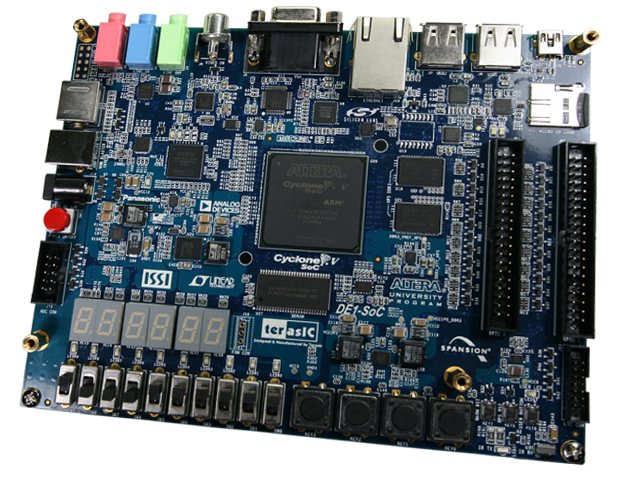
\includegraphics[width=\textwidth]{pictures/fpga-board.jpg}
\caption{Płytka Terasic DE1-SOC \cite{plytka}}
\label{fig:fpga-board}
\end{figure}


Układ FPGA znajdujący się na wybranej płytce posiada zintegrowany procesor ARM (HPS, ang. \textit{Hard Processor System}). Dzięki temu możliwe jest m.in. uruchomienie systemu operacyjnego Linux. Między programowalną częścią układu a procesorem ARM jest interfejs umożliwiający szybką komunikacją. Pozwala to m.in. na skonfigurowanie układu FPGA jako karty graficznej i korzystania z systemu operacyjnego w trybie graficznym. Istotnymi dla tego projektu właściwościami takiego połączenia są:
\begin{enumerate}
\item Nie wszystkie urządzenia peryferyjne są podłączone bezpośrednio do programowalnej części układu FPGA -- niektóre są podłączone do procesora ARM. Powoduje to, że aby uzyskać dostęp do ich sygnałów z FPGA, wymagana jest dodatkowa konfiguracja multipleksacji pinów przeprowadzona przez preloader podczas procedury startowej. Konwerter USB-UART firmy FTDI jest przykładem układu peryferyjnego, który jest podłączony do procesowa ARM i wymaga takie konfiguracji.
\item Obecność procesora ARM umożliwia wykonanie przy starcie płytki skryptów zdefiniowanych przez użytkownika i umieszczonych na karcie SD. Przykładem zastosowania jest programowanie układu FPGA przy starcie układu.
\end{enumerate}


\subsubsection{Fazy startowe}
Proces startowania płytki składa się z czterech faz \cite[p. 1068]{altera-vol3}. Dwie pierwsze fazy są konieczne do prawidłowego zainicjowania układu FPGA oraz zintegrowanego procesora ARM. Dwie kolejne fazy są opcjonalne. Kod wykonywalny fazy BootROM znajduje się w zintegrowanej pamięci HPS. Kod pozostałych faz musi być dostarczony przez użytkownika, np. w postaci plików zapisanych na karcie SD.
\begin{enumerate}[noitemsep]
\item BootROM -- przeprowadza minimalną konfigurację oraz ładuje preloader do zintegrowanej pamięci RAM.
\item Preloader -- inicjalizacja SDRAM, konfiguracja multipleksacji pinów HPS I/O, załadowanie boot loadera do pamięci SDRAM.
\item Boot Loader (U-Boot) -- wykonuje zdefiniowane przez użytkownika skrypty startowe, inicjuje start systemu operacyjnego.
\item Operating System -- uruchomienie oraz działanie systemu operacyjnego.
\end{enumerate}


\subsection{Transmisja UART}
\label{sec:uart-parametry}
Protokół UART (ang. \textit{Universal Asynchronous Receiver and Transmitter}) jest protokołem umożliwiającym dwustronną szeregową transmisję danych. Wykorzystywany jest m.in. w standardzie RS-232. Najprostsza wersja składa się z dwóch sygnałów RX i TX, po jednym dla każdego z kierunków transmisji. UART umożliwia wybór parametrów transmisji. W tym projekcie zostały użyte następujące parametry:
\begin{enumerate}[noitemsep]
\item Szybkość transmisji: 115200 baud
\item 1 bit startu
\item 1 bit stopu
\item Brak kontroli bitu parzystości -- kontrola poprawności odebranych danych realizowana jest przy pomocy obliczania sumy kontrolnej CRC16 (ang. \textit{cyclic redundancy check}) całych bloków danych (patrz rozdział \ref{sec:crc16}).
\item Bity w bajcie przesyłane są od najmłodszego -- \textit{LSB first}
\end{enumerate}

\begin{figure}[!h]
\centering
\begin{tikztimingtable}[timing/wscale=3.3]
  \textit{CLK\_UART} & c cc        cc         cc         cc         cc         cc         cc         cc         cc         cc       c \\
  \textit{RX}        & u J{Start}  D{Data[0]} D{Data[1]} D{Data[2]} D{Data[3]} D{Data[4]} D{Data[5]} D{Data[6]} D{Data[7]} K{Stop}  u \\
\extracode
\tablerules
\end{tikztimingtable}
\caption{Format ramki UART}
\label{fig:uart-frame}
\end{figure}

\newpage
Wybrana konfiguracja parametrów powoduje, że ramka UART ma format przedstawiony na rysunku \ref{fig:uart-frame}. Pozwala ona również na transmisję z prędkością:

\begin{equation*}
115200 BAUD * 8 / 10 = 92160 b/sek
\end{equation*}

Po uwzględnieniu narzutu związanego z kontrolą poprawniści CRC16 (2 bajty CRC + 1 bajt ACK na każdy 128-bajtowy blok danych, rozdz. \ref{sec:crc16}), kanał komunikacyjny będzie w stanie przesyłać dane z prędkością:

\begin{equation*}
92160 b/sek * 128 / 131 = 90049 b/sek \approx 11,2 KB/sek 
\end{equation*}

Taka prędkość transmisji pozwoli na zaszyfrowanie pliku o wielkości 1MB w czasie 90 sekund. Występujące błędy transmisji dodatkowo spowolnią szyfrowanie.

\subsection{Kolejność bitów i bajtów}
\begin{itemize}
\item Podczas transmisji danych bity w bajcie przesyłane są od najmłodszego do najstarszego (\textit{LSB first}), ponieważ jest to domyślny sposób wykorzystywany przez sterownik UART w systemie operacyjnym Linux.
\item Podczas transmisji danych bajty w bloku są przesyłane zgodnie z kolejnością ich odczytu i zapisu na dysku -- pierwszy odczytany (najstarszy) bajt jest przesyłany jako pierwszy. Taki sposób formowania bloków jest również używany przez program \textit{openssl}.
\item Moduły szyfrujące i deszyfrujące AES operują na bajtach, w których najmłodszy (pierwszy odebrany lub wysłany) bit ma numer 0, co jest zgodne ze standardem AES.
\item Moduły szyfrujące i deszyfrujące AES operują na blokach, w których najstarszy (pierwszy odebrany lub wysłany) bajt ma numer 0, co jest zgodne ze standardem AES.
\end{itemize}

\subsection{Przyjęte konwencje}

W celu poprawy czytelności rysunków przebiegów czasowych w dokumentacji będzie pojawiał się umowny zegar \textit{CLK\_UART}. Dla wygody czytelnika została również wprowadzona konwencja kolorystyczna sygnałów.

\subsubsection{Zegar \textit{CLK\_UART}}
Głównym sygnałem zegarowym układu jest \textit{CLK\_16} (rozdz. \ref{sec:clk-16}). Ze względu na jego szybką zmienność przedstawienie go na niektórych przebiegach czasowych nie jest możliwe. W takich przypadkach będzie on zastąpiony umownym sygnałem \textit{CLK\_UART} o częstotliwości $f_{CLK\_UART}$.
\begin{equation*}
f_{CLK\_UART} = \frac{f_{CLK\_16}}{16} = UART\_BAUD\_RATE
\label{eq:clk-uart-freq}
\end{equation*}
gdzie \textit{UART\_BAUD\_RATE} jest szybkością transmisji sygnału UART wyrażoną w baudach. 

\begin{figure}[!h]
\centering
\begin{tikztimingtable}
  \textit{CLK\_16}   & c 16{cc}     16{cc}       7{c}       \\
  \textit{CLK\_UART} & c 2{16c}     2{16c}       7c         \\
\extracode
\tablerules
\vertlines[red]{0.5}
\vertlines[red]{8.5}
\vertlines[red]{16.5}
\vertlines[red]{24.5}
\vertlines[red]{32.5}
\end{tikztimingtable}
\caption{Relacja między zegarami \textit{CLK\_16} i \textit{CLK\_UART}}
\label{fig:clks-relation}
\end{figure}

Zbocza rosnące i malejące zegara \textit{CLK\_UART} będą się pokrywać ze zboczami rosnącymi zegara \textit{CLK\_16} (rys. \ref{fig:clks-relation}). 

\subsubsection{Konwencje kolorystyczne i nazewnicze sygnałów}
W tekscie dokumentacji oraz na przebiegach nazwy sygnałów wejściowych będą zaznaczane kolorem \insignal{zielonym}, a wyjściowych kolorem \outsignal{czerwonym}. Sygnał \textit{CLK\_UART}, który zawsze będzie występował jako sygnał wejściowy, będzie zaznaczany kolorem \helpsignal{pomarańczowym}.


Wektory sygnałów będą oznaczane poprzez dodanie ich zakresu w nawiasach kwadratowych na końcu nazwy, np. \textit{BYTE[7:0]} jest wektorem ośmiu sygnałów.


Ze względu na fakt, że niektóre sygnały zmieniają się o wiele szybciej od innych, poprawne zachowanie wszystkich proporcji czasowych na rysunkach jest niemożliwe. Przykładem jest sygnał \textit{BYTE[7:0]}, który przyjmuje wartość {'1'} na czas 2048 razy mniejszy niż czas w którym sygnał \textit{AES\_BLOCK[127:0]} pozostaje niezmienny. W takich sytuacjach, proporcje czasowe przedstawione na przebiegach mogą być zaburzone. Kolejność występowania zdarzeń (zmian wartości sygnałów) będzie bezwzględnie zachowana.


Wszystkie moduły mają zaimplementowany asynchroniczny sygnał \insignal{RESET\_N}. W celu poprawy czytelności nie będzie on uwzględniany na przebiegach czasowych oraz schematach.